A Organização das Nações Unidas (ONU) é uma instituição intergovernamental fun- dada em 1945, após a Segunda Guerra Mundial. A instituição foi estabelecida com o propósito de trabalhar em prol da paz, do desenvolvimento e da segurança global. Atualmente, a organi- zação conta com 193 países membros voluntários que constituem a Assembleia Geral, órgão responsável pelo desenvolvimento das políticas. Em 2015, os 193 Estados-membros da ONU reuniram-se para estabelecer um novo documento intitulado "Transformando o Nosso Mundo: A Agenda 2030 para o Desenvolvimento Sustentável". Esta agenda é composta por 17 objetivos que abrangem áreas desde o desenvolvimento sustentável até a promoção da saúde da população. No Brasil, é de extrema importância que haja um esforço coletivo para acelerar o processo de alcançar os 17 objetivos. Este trabalho busca contribuir para atingir uma das metas propostas na Agenda 2030, baseando-se no seguinte objetivo: combater doenças transmissíveis, tanto em número de casos quanto em número de óbitos, associado à terceira meta, que promove saúde e bem-estar. \cite{1} 

A palavra epidemia indica a proliferação de uma doença, nesse caso, o aumento do número de casos de determinada doença, que vai muito além do esperado em diversas regiões, cidades ou estados, mas sem atingir níveis globais. \cite{2}. O território brasileiro foi alvo de enfermidades classificadas como epidemias ao longo dos anos, o que foi extremamente prejudicial à população brasileira devido à rápida contaminação e ao elevado número de óbitos. Ao longo do século XXI, algumas doenças passaram a preocupar a população brasileira, entre elas a dengue.

A dengue é uma doença transmitida pela picada do mosquito Aedes aegypti e pode variar entre três categorias: dengue clássica (DC); febre hemorrágica da dengue (FHD); e choque hemorrágico da dengue (CHD). Além disso, ao longo dos anos, diferentes sorotipos foram introduzidos: DENV-1, DENV-2, DENV-3 e DENV-4, que apresentam diferentes materi- ais genéticos e linhagens. \cite{3}. A dengue se mostrou preocupante nos últimos meses devido aos números de contaminados e de óbitos. Foram registradas 1.020 mortes por dengue e, ao todo, 2.671.332 infecções neste ano no Brasil. \cite{4}

A dengue é classificada como um arbovírus, ou seja, um grupo de doenças causadas por vírus transmitidos por artrópodes. A doença é transmitida por mosquitos fêmeas contami- nados da espécie Aedes aegypti, que necessitam do sangue humano para o desenvolvimento de seus ovos e metabolismo. Não há transmissão por meio do contato com um doente, ou de fontes de água e alimento. \cite{3} A fêmea se alimenta de sangue no início da manhã e no final da tarde, o que não impede que a picada aconteça em outros horários. \cite{5}. Alguns fatores podem influenciar a proliferação e transmissão da dengue, como a precipitação, a temperatura e a urbanização não planejadas, já que o vetor prefere depositar seus ovos em recipientes artificiais que contenham água, principalmente em tambores, barris e pneus, encontrados dentro e nas proximidades de residências, escolas e locais de trabalho. Os ovos do mosquito têm a capacidade de resistir a condições ambientais secas por mais de um ano. Essa é uma das estratégias mais importantes que a espécie utiliza para sua sobrevivência e disseminação. Esses insetos também são responsáveis pela transmissão da febre amarela, Chikungunya e Zika. \cite{6}.
\begin{figure}[H]
    \centering
    \caption{Pernilongo X Mosquito da dengue}
    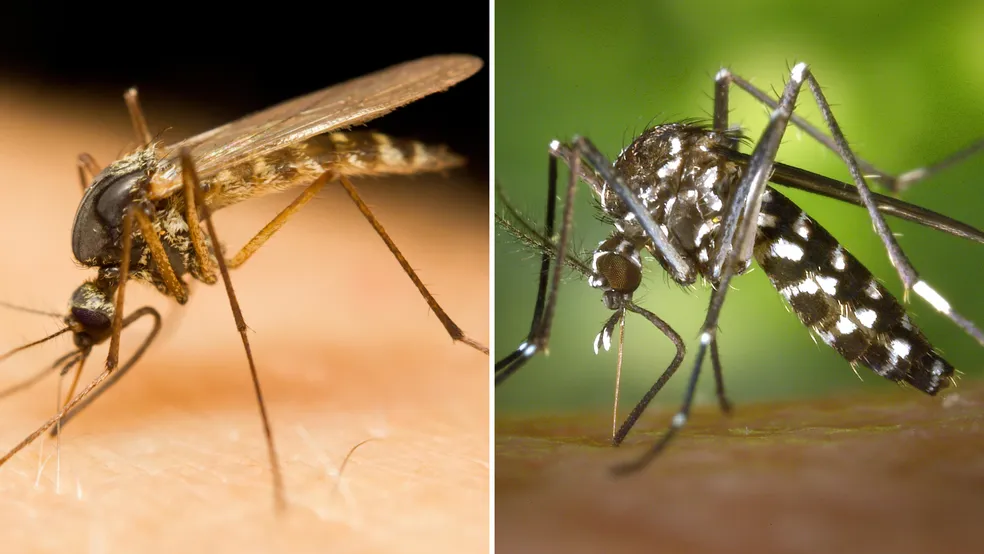
\includegraphics[width=0.5\linewidth]{Illustrations/aedes.png}
    \caption*{\textbf{Fonte: Globo Rural, 2023.}}
    \label{fig:enter-label}
\end{figure}
A enfermidade varia entre formas assintomáticas ou graves, levando a óbito. A maneira como a doença se manifesta em humanos pode variar de acordo com alguns fatores, como o vírus envolvido, infecção anterior pelo vírus da dengue e aspectos individuais, como doenças crônicas. O homem infectado pode apresentar sintomas de 2 a 7 dias, como febre, dor de cabeça, dor ao movimentar os olhos e dores musculares. Além destes, manchas vermelhas no corpo, vômitos e sangramentos no nariz ou nas gengivas podem ser um alerta para dengue hemorrágica. Os quatro sorotipos da dengue podem produzir formas assintomáticas e graves, mas os sorotipos 2 e 3 são considerados mais severos. \cite{7}. 
\begin{figure}[H]
    \centering
    \caption{Sintomas de dengue}
    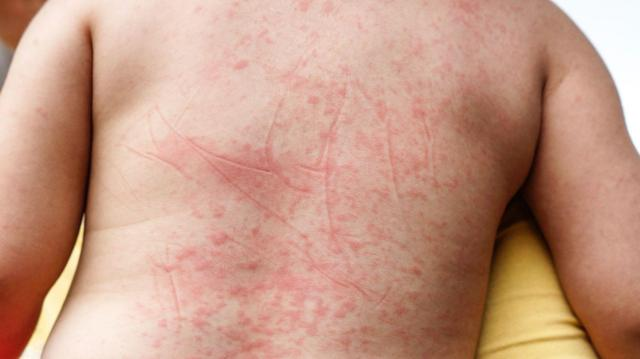
\includegraphics[width=0.5\linewidth]{Illustrations/sintomas.png}
    \caption*{\textbf{Fonte: BBC News Brasil, 2024.}}
    \label{fig:enter-label}
\end{figure}
Não há um tratamento específico ou remédios específicos para a dengue. O que pode ser feito é procurar suporte médico assim que os sintomas se manifestem para que ocorra um tratamento oportuno, a fim de minimizar o número de óbitos. \cite{8}. Uma alternativa é conter o criadouro do Aedes aegypti de maneira coletiva para reduzir a transmissão, eliminando água parada em pneus, garrafas vazias, potes, vasos de plantas ou qualquer outro objeto em que possa acumular água, além de realizar a limpeza da caixa d’água. \cite{9}.

Existem dificuldades relacionadas ao poder público que aceleram a transmissão da dengue. A primeira diz respeito ao fluxo rural-urbano ocorrido nos últimos anos, resultando em uma população de 124,1 milhões de pessoas nos centros urbanos até 2022. \cite{10}. Diante desse cenário, há uma falta de condições de habitação satisfatórias e saneamento básico por parte das cidades. Por essa razão, parte da população é submetida a um abastecimento de água e coleta de resíduos irregulares. Sem alternativas, a solução encontrada por essas pessoas é armazenar água para consumo, fator que favorece a proliferação do vetor. A produção de veículos também contribui para um maior número de pneus usados dispersos no meio ambiente. Outro empecilho referente ao poder público é a regularização do abastecimento de água e coleta de lixo em locais onde essas atividades não foram satisfatórias após o processo de fluxo rural-urbano, particularmente em comunidades carentes. O último ponto trata-se da pobre inspeção residencial, que abrange o cuidado ou eliminação de reservatórios potenciais do vetor. \cite{11}. 

Atualmente, os agentes de saúde já contribuem no combate às epidemias de dengue, alertando os moradores sobre os riscos e tratamentos dessa enfermidade, combatendo a eliminação de focos do Aedes aegypti e monitorando possíveis casos. Ademais, existem pesquisas dedicadas em tratar a dengue como uma endemia, realizando a contabilização de casos em distintas categorias por meio de gráficos ou mapas. No entanto, observa-se que os dados fornecidos por meio de aplicações já existentes representam apenas a última atualização, a qual pode ter ocorrido há três semanas, por exemplo \cite{20}. \cite{21}. \cite{22}. \cite{23}. Entretanto, há a carência de dados disponibilizados em tempo real para que os locais de foco das doenças sejam tratados de forma eficaz antes que a situação se agrave.

Dessa forma, a proposta do projeto é desenvolver um sistema de identificação de áreas de risco de dengue no Brasil. A aplicação consiste em desenvolver um sistema dedicado aos agentes de saúde, que poderão acessar um mapa para cadastrar o endereço residencial e o local de trabalho ou estudo de pessoas infectadas, além da localização de áreas com foco de dengue, como um pneu com água acumulada, por exemplo. Por outro lado, o gestor da equipe de agentes de saúde poderá ter acesso ao mapa de calor com os dados atualizados em tempo real, com o intuito de que a equipe de dedetização seja enviada para o tratamento do local.

A inteligência artificial (IA) é uma tecnologia que simula a capacidade humana de pensar, aprender e resolver problemas. Ela é usada em diversos campos para processar grandes quantidades de dados, tomar decisões rápidas e precisas, criar algoritmos e programas de computador. \cite{24}.

Com o intuito de promover a eficácia do sistema, o projeto em questão busca incluir a IA para cruzar as regiões afetadas de forma que estas sejam disponibilizadas de forma prioritária, ou seja, cada ponto representado no mapa receberá um nível de intensidade para determinar a ordem do processo de dedetização do ambiente e conter o avanço das doenças. Assim, a visualização dos dados e a eficácia no auxílio ao combate das epidemias de dengue podem ser aprimoradas. Este projeto é desenvolvido em colaboração com a prefeitura da cidade à qual se destina


